\documentclass[conference]{IEEEtran}
\usepackage[utf8]{inputenc}
\usepackage[spanish,english]{babel}
\usepackage{cite}
\usepackage{amsmath,amssymb,amsfonts}
\usepackage{graphicx}
\usepackage{textcomp}
\usepackage{xcolor}
\usepackage{hyperref}

% Path de imágenes
\graphicspath{{./imagenes/}}

\begin{document}

\title{Diseño de un Sistema de Radar Acústico para Estimación de Distancia}

\author{
    \IEEEauthorblockN{José Andrés Solano Mora}
    \IEEEauthorblockA{\textit{Escuela de Ingeniería en Computadores} \\
    \textit{Instituto Tecnológico de Costa Rica}\\
    Cartago, Costa Rica}
}

\maketitle

% --- ABSTRACT ---
\begin{otherlanguage}{english}
\begin{abstract}
This paper presents the design and implementation of an acoustic radar system for object detection and distance estimation using continuous acoustic signal processing. The system employs a acoustic transmitter, a microphone receiver, and a microcontroller for signal digitization and processing. Fast Fourier Transform (FFT) algorithms and cross-correlation techniques are applied to calculate the Time-of-Flight (ToF) of the reflected acoustic signals. Experimental results demonstrate the performance of FFT-based correlation compared to direct time-domain implementation, validating its effectiveness in noisy environments.
\end{abstract}

\begin{IEEEkeywords}
Acoustic Radar, Fast Fourier Transform (FFT), Cross-Correlation, Time of Flight (ToF), Digital Signal Processing.
\end{IEEEkeywords}
\end{otherlanguage}

% --- INTRODUCCIÓN ---
\section{Introducción}
\selectlanguage{spanish}
En el campo del procesamiento digital de señales, la estimación de distancia mediante ondas acústicas representa una aplicación práctica de los sistemas lineales e invariantes en el tiempo (LTI)~\cite{oppenheim2009}. Este proyecto abarca la concepción, simulación e implementación de un radar acústico capable de calcular el tiempo de vuelo ($\text{ToF}$) de una señal conocida tras reflejarse en un objeto.

La organización del presente documento se estructura de la siguiente manera: La Sección~\ref{sec:marco_teorico} presenta la revisión bibliográfica sobre transformación de Fourier y correlación. La Sección~\ref{sec:resultados} detalla los experimentos en simulación y los resultados en hardware. Finalmente, las Secciones~\ref{sec:conclusiones} y~\ref{sec:recomendaciones} presentan las conclusiones y recomendaciones.

% --- MARCO TEÓRICO ---
\section{Marco Teórico y Revisión Bibliográfica}
\label{sec:marco_teorico}
\selectlanguage{spanish}
El cálculo del tiempo de retardo entre una señal transmitida $x(t)$ y una señal recibida $y(t)$ se fundamenta en la correlación cruzada $R_{xy}(\tau)$, definida formalmente como:
\begin{equation}
R_{xy}(\tau) = \int_{-\infty}^{\infty} x(t) y(t + \tau) \, dt
\end{equation}

A través del teorema de convolución, la correlación en el dominio del tiempo equivale a una multiplicación en el dominio de la frecuencia:
\begin{equation}
\mathcal{F}\{R_{xy}(\tau)\} = X^*(f) \cdot Y(f)
\end{equation}
donde $X^*(f)$ denota el complejo conjugado de la Transformada de Fourier de la señal emitida.

% --- RESULTADOS Y ANÁLISIS ---
\section{Resultados y Análisis de Resultados}
\label{sec:resultados}
\selectlanguage{spanish}

\subsection{Experimentos con FFT y DFT}
Se comparó el desempeño computacional entre la DFT directa $O(N^2)$ y el algoritmo FFT Radix-2 $O(N \log N)$. La Fig.~\ref{fig:tiempos} ilustra la diferencia en tiempo de ejecución para distintos tamaños de muestra $N$.

\begin{figure}[htbp]
    \centering
    %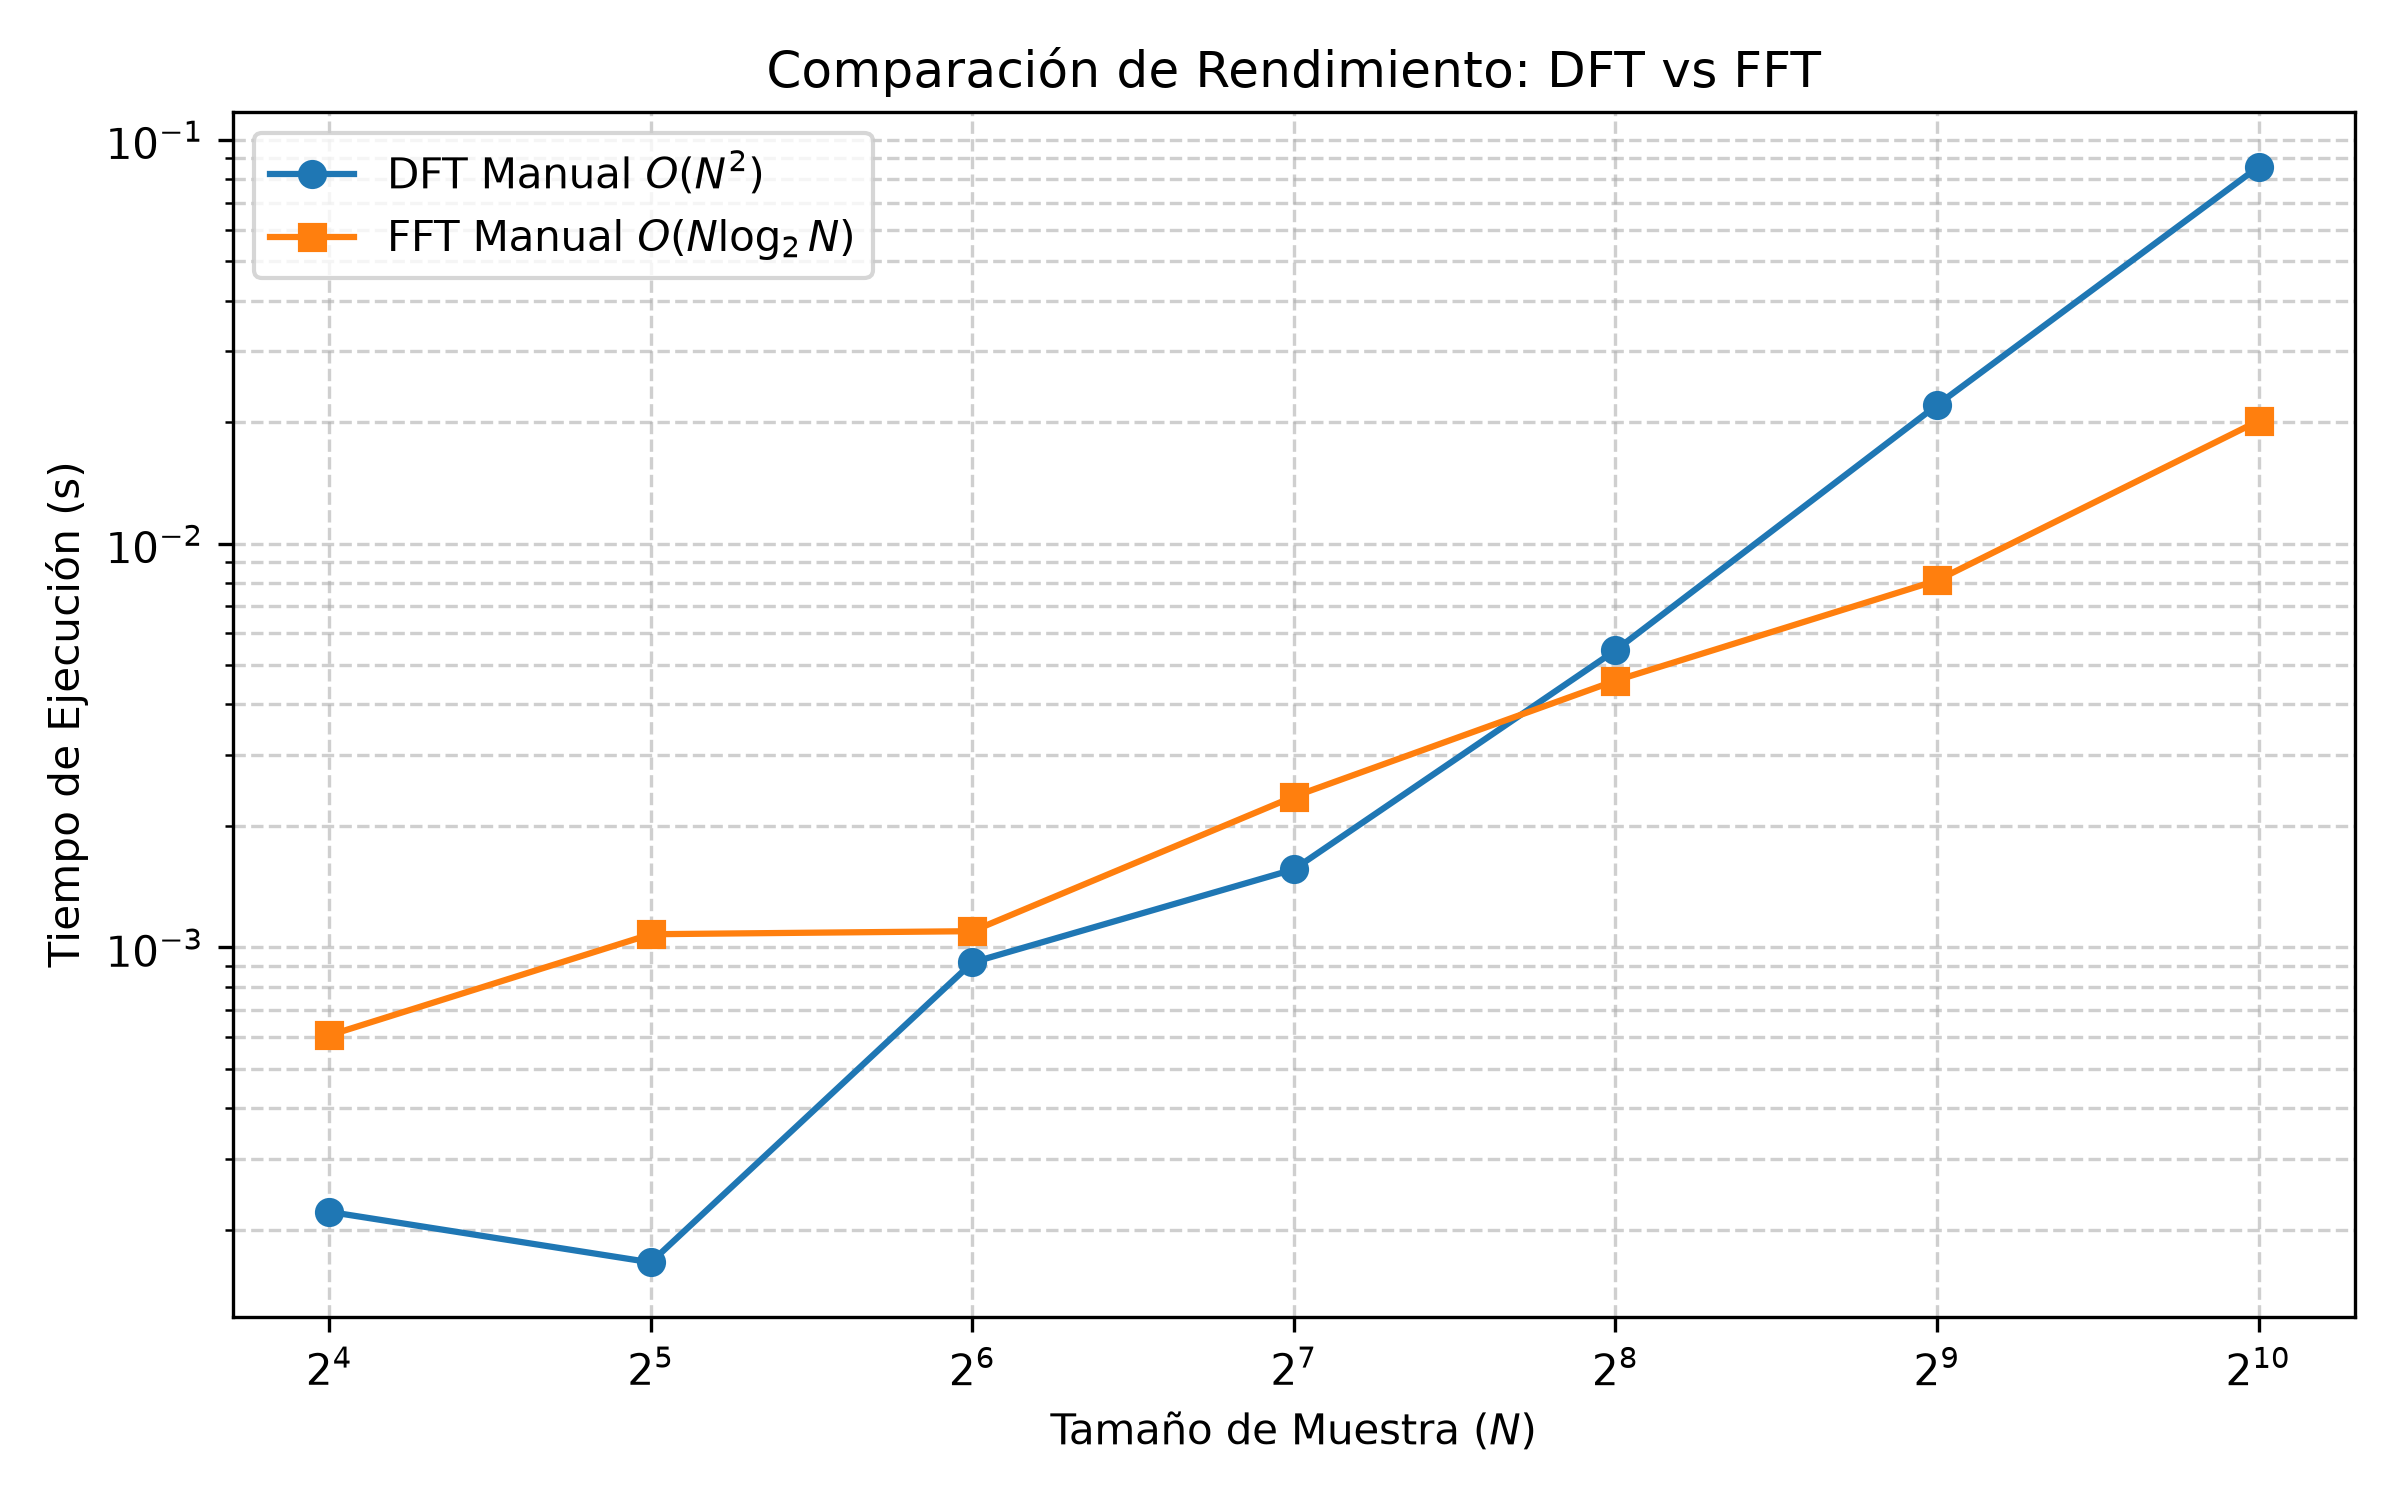
\includegraphics[width=0.45\textwidth]{etapa2_tiempos_dft_fft.png}
    \caption{Comparación de tiempos de ejecución entre DFT y FFT.}
    \label{fig:tiempos}
\end{figure}

\subsection{Detección de Ecos y Correlación}
Mediante el uso de impulsos tipo \textit{Chirp}, se identificó el retardo del eco en presencia de ruido blanco aditivo (AWGN). La distancia $d$ se determinó mediante:
\begin{equation}
d = \frac{v_s \cdot \text{ToF}}{2}
\end{equation}
donde $v_s \approx 343 \text{ m/s}$ representa la velocidad del sonido en el aire a temperatura ambiente.

% --- CONCLUSIONES ---
\section{Conclusiones}
\label{sec:conclusiones}
\selectlanguage{spanish}
La implementación de la correlación cruzada en el dominio de la frecuencia mediante la FFT redujo significativamente el costo computacional en comparación con la implementación directa en el tiempo. La utilización de señales moduladas en frecuencia (chirp) demostró una mayor robustez frente al ruido ambiental en la detección del tiempo de vuelo.

% --- RECOMENDACIONES ---
\section{Recomendaciones}
\label{sec:recomendaciones}
\selectlanguage{spanish}
Se recomienda acondicionar analógicamente la señal del micrófono mediante un filtro pasa-banda antes del proceso de digitalización con el ADC para evitar el solapamiento de frecuencias y reducir interferencias de baja frecuencia.

% --- BIBLIOGRAFÍA ---
\bibliographystyle{IEEEtran}
\bibliography{referencias}

\end{document}